\chapter{Statistics: Hypothesis Testing}
\section{General Information}
\begin{definition}{}{}
  The \emph{null hypothesis} \(H_0\) and \emph{alternative hypothesis} \(H_1\) are the hypotheses that we hope to reject and accept, respectively. 
\end{definition}
\begin{note}
  To check we have correctly stated the hypotheses in our hypothesis test, ensure that they are contrasting. For example, we are testing A's claim that \(\mu>\mu_0\):

  \begin{minipage}{0.45\textwidth}
    \vspace{\baselineskip}
    \begin{tabular}{|ll|}
      \hline
      Test & \(H_0\colon\mu=\mu_0\) (A's claim is false)\\
      against &\(H_1\colon\mu<\mu_0\) (A's claim is false)\\
      \multicolumn{2}{|l|}{at the \(100\alpha\%\) significance level.}\\
      \hline
    \end{tabular}

    \vspace{\baselineskip}
    Both hypotheses result in A's claim being false. Hence, the hypotheses have been stated erroneously \textcolor{red}{\(\times\)}.  
  \end{minipage}%
  \hfill
  \begin{minipage}{0.45\textwidth}
    \vspace{\baselineskip}
    \begin{tabular}{|ll|}
      \hline
      Test & \(H_0\colon\mu=\mu_0\) (A's claim is false)\\
      against &\(H_1\colon\mu>\mu_0\) (A's claim is true)\\
      \multicolumn{2}{|l|}{at the \(100\alpha\%\) significance level.}\\
      \hline 
    \end{tabular}  

    \vspace{\baselineskip}
    The hypotheses are contrasting. So, they have been correctly stated \textcolor{green!70!black}{\checkmark}. 
    \vspace{\baselineskip}
  \end{minipage}
\end{note}
\begin{stbox}{General Information}
  \begin{itemize}
    \item Without going into details, a \emph{critical region} \(C\) is just a set that defines the decision rule / test 
    \begin{center}
      Reject \(H_0\) (Accept \(H_1\)) \quad if \((X_1,X_2,\dots,X_n)\in C\),
    \end{center}
    for any random sample \(X_1,X_2,\dots,X_n\) from the distribution of a random variable \(X\).
  \end{itemize}
\end{stbox}
\begin{definition}{}{}
  The \emph{significance level} \(100\alpha\%\) of a test is the probability of rejecting \(H_0\) when it is in fact true. i.e. \(\alpha=\Prob(H_0\text{ is rejected}\,\vert\,H_0\text{ is true})\).
\end{definition}
\begin{note}
  Explain, in context, the meaning of `at the \(\alpha\%\) level of significance'.
  \begin{center}
    \parbox{0.9\textwidth}{
      The probability that we conclude [\(H_1\) in context], when actually [\(H_0\) in context], is \(\alpha\%\).
    }
  \end{center}
\end{note}
\begin{definition}{}{}
  The \emph{\(p\)-value} is the lowest level of significance for which the null hypothesis will be rejected. In other words, for the null hypotheses
    \begin{center}
      \begin{enumerate*}[label=(\alph*),itemjoin={\quad}]
        \item \(\mu<\mu_0\),
        \item \(\mu \neq \mu_0\),
        \item \(\mu>\mu_0\),
      \end{enumerate*}
    \end{center}
    we have
    \begin{center}
      \begin{enumerate*}[label=(\alph*),itemjoin={\quad}]
        \item \(p\text{-value}\coloneq\Prob(Z\leq z_\text{calc})\),
        \item \(p\text{-value}\coloneq\Prob(\lvert Z \rvert\geq \lvert z_\text{calc} \rvert)\),
        \item \(p\text{-value}\coloneq\Prob(Z\geq z_\text{calc})\).
      \end{enumerate*}
    \end{center}
\end{definition}
\begin{note}
  Explain what the \(p\)-value means in context.
  \begin{center}
    \parbox{0.9\textwidth}{
      The \(p\)-value is the least level of significance to conclude that [\(H_1\) in context].
    }
  \end{center}
\end{note}
\begin{stbox}{}
  \begin{itemize}
    \item One sample \(z\)-test. There are various combinations of assumptions for which this test applies. For brevity, we shall avoid restating it, instead directing the reader to table \ref{Table:Summary table for one-sample hypothesis testing.}.
    \begin{enumerate}
      \item Let [\(X\) in context] and \(\mu\) be the population mean.
      \item 
      \begin{tabular}{|ll|}
        \hline
        Test & \(H_0\colon\mu=\mu_0\)\\
        against &\(H_1\colon\) 
        \begin{enumerate*}[itemjoin={\quad}]
          \item \(\mu<\mu_0\),
          \item \(\mu \neq \mu_0\),\quad or
          \item \(\mu>\mu_0\),
        \end{enumerate*}\\
        \multicolumn{2}{|l|}{at the \(100\alpha\%\) significance level.}\\
        \hline
      \end{tabular}
      \item Under \(H_0\), we have \(\widebar{X}\sim \Normal(\mu_0,\hat{\sigma}^2/n)\) approximately. Or, if \(\sigma^2\) is known exactly, then by CLT \(\widebar{X}\sim \Normal(\mu_0,\sigma^2/n)\) approximately.
      \item Test statistic: 
      \[Z=\frac{\widebar{X}-\mu_0}{\sigma/\sqrt{n}}\sim\Normal(0,1).\]
    \end{enumerate}
      \begin{minipage}[t]{0.45\textwidth}
        \begin{enumerate}
          \setcounter{enumi}{3}
          \item Find \(z_{1-\alpha}\) or \(z_{1-\alpha/2}\), which satisfies
          \begin{enumerate}
            \item \(\Prob(Z<z_{1-\alpha})=\alpha\), 
            \item \(\Prob(-z_{1-\alpha/2}<Z<z_{1-\alpha/2})=1-\alpha\), or
            \item \(\Prob(Z>z_{1-\alpha})\).
          \end{enumerate}
          \item Find the test statistic value 
          \[z_\text{calc}=\frac{\hat{\mu}-\mu_0}{\sigma/\sqrt{n}}.\]
          \item Reject \(H_0\) iff 
          \begin{enumerate}
            \item \(z_\text{calc}<z_{1-\alpha}\),
            \item \(\lvert z_\text{calc} \rvert>z_{1-\alpha/2}\), or
            \item \(z_\text{calc}>z_{1-\alpha}\).
          \end{enumerate}
        \end{enumerate}
      \end{minipage}
      \begin{minipage}[t]{0.45\textwidth}
        \begin{enumerate}
          \setcounter{enumi}{3}
          \item Find the \(p\)-value using GC.
          \item Reject \(H_0\) iff \(p\)-value is less than \(\alpha\).
        \end{enumerate}
        \vfill
        \begin{flushright}
          \begin{minipage}{0.8\textwidth}
            \begin{GCSkills}{}
              Calculating the \(p\)-value of a sample.
              \begin{center}
                \texttt{stat \(\Longrightarrow\) TESTS \(\Longrightarrow\) 1:Z-Test\dots}
              \end{center}
            \end{GCSkills}
          \end{minipage}
        \end{flushright}
      \end{minipage}
      \begin{enumerate}
        \item[7.] Since\quad
        \begin{enumerate*}[label=(\alph*),itemjoin={\quad}]
          \item \(z_\text{calc}<z_{1-\alpha}\),
          \item \(\lvert z_\text{calc} \rvert>z_{1-\alpha/2}\),
          \item \(z_\text{calc}>z_{1-\alpha}\),\quad or\quad \(p\text{-value}<\alpha\),
        \end{enumerate*}
        we reject \(H_0\). There is sufficient evidence at the significance level \(100\alpha\%\) that [\(H_1\) in context].

        \emph{Note.} For \emph{not} rejecting \(H_0\), simply change to the appropriate inequality (such that \(z_\text{calc}\) is outside the critical region) and write ``insufficient'' instead of ``sufficient''.
      \end{enumerate}
      \item If we have a null hypothesis, such as
      \begin{center}
        \(H_0\colon\mu\leq\mu_0\)\quad or\quad \(H_0\colon\mu\geq\mu_0\),
      \end{center}
      we can just use \(H_0\colon\mu=\mu_0\) instead.
  \end{itemize}
\end{stbox}
% \begin{definition}{}{}
%   We say a critical region \(C\) is of \emph{size} \(\alpha\) if 
%   \[\alpha=\max_{\theta\in\omega_0}P_\theta[(X_1,X_2,\dots,X_n)\in C].\]
%   In our syllabus, \(\alpha\cdot100\%\) is called the \emph{significance level}.
% \end{definition}
\begin{note}
  Explain why there is no need to assume that the distribution of \(X\) is normal/know anything about the population distribution of \(X\).
  \begin{center}
    \parbox{0.9\textwidth}{
      As the \hly{sample size \(n\) is large}, by the \hly{Central Limit Theorem}, the \hly{sample mean} of [random variable \(X\) in context] will \hly{approximately follow a normal distribution}.
    }
  \end{center}
  \emph{Note.} Spell ``Central Limit Theorem'' and ``the sample mean'' out \emph{in full}. Do not use CLT or \(\widebar{X}\) for this question.
\end{note}
\begin{definition}{}{}
  A random variable \(X\) follows Student's \(t\)-distribution with \(\nu\) degrees of freedom iff its pdf is
  \[f(t)=\frac{\Gamma{\left( \frac{\nu+1}{2} \right)}}{\sqrt{\pi\nu}\ \Gamma{\left( \frac{\nu}{2} \right)}}\left( 1+\frac{t^2}{\nu} \right)^{-\frac{1}{2}(\nu-1)}.\]
  This is denoted by \(X\sim t(\nu)\).
\end{definition}
\begin{figure}[H]
  \centering
  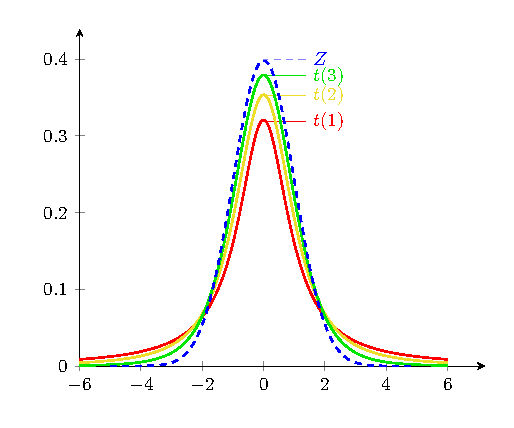
\includegraphics[width=0.5\textwidth]{../Diagrams/t-distribution/t-distributon.pdf}
  \caption{Student's \(t\)-distribution compared to the standard normal distribution.}
  \label{Fig:Student}
\end{figure}
\begin{stbox}{}
  \begin{itemize}
    \item Properties of Student's \(t\)-distribution.
    \begin{enumerate}
      \item It is continuous and symmetric about the vertical axis, i.e. \(t=0\).
      \item From Figure \ref{Fig:Student}, we see that the \(t\)-distribution has a flatter peak and fatter tails, than the standard normal distribution.
      \item As \(\nu\to\infty\), we have \(t(\nu)\to\Normal(0,1)\).
    \end{enumerate}
    \item Let \(T\sim t(n-1)\) and \(t_{(n-1,1-\alpha/2)}\) be such that \(\Prob{\left(-t_{(n-1,1-\alpha/2)}<T<t_{(n-1,1-\alpha/2)}\right)}=1-\alpha\). A \((1-\alpha)100\%\) confidence interval, for the population mean \(\mu\) of \(T\), is
    \[\left( \widebar{x}-t_{(n-1,1-\alpha/2)}\frac{s}{\sqrt{n}}\,,\ \widebar{x}-t_{(n-1,1-\alpha/2)}\frac{s}{\sqrt{n}} \right).\]
    \item Suppose we are conducting the following test:
    \begin{center}
      \begin{tabular}{|ll|}
        \hline
        Test & \(H_0\colon\mu=\mu_0\)\\
        against &\(H_1\colon\mu\neq\mu_0\)\\
        \multicolumn{2}{|l|}{at a \(100\alpha\%\) significance level.}\\
        \hline
      \end{tabular}
    \end{center}
    Then, we reject \(H_0\) iff the appropriate symmetric interval (\(z\) or \(t\)-interval) does \emph{not} contain \(\mu_0\). 
  \end{itemize}
\end{stbox}
\begin{GCSkills}{}
  Calculating the symmetric \(t\)-confidence interval, for the population mean, of a random variable following Student's \(t\)-distribution.
  \begin{center}
    \texttt{stat} \(\Longrightarrow\) \texttt{TESTS} \(\Longrightarrow\) \texttt{8:TInterval\dots} 
  \end{center}
\end{GCSkills}
\begin{stbox}{}
  \begin{itemize}
    \item A one sample \(t\)-test.
    % We use this test when \emph{the population variance is unknown} and the sample size is small.
    Again, see table \ref{Table:Summary table for one-sample hypothesis testing.} for the necessary assumptions.
    \begin{enumerate}
      \item Let [\(X\) in context], \emph{which we assume to be normally distributed}, and \(\mu\) be the population mean.
      \item 
      \begin{tabular}{|ll|}
        \hline
        Test & \(H_0\colon\mu=\mu_0\)\\
        against &\(H_1\colon\) 
        \begin{enumerate*}[itemjoin={\quad}]
          \item \(\mu<\mu_0\),
          \item \(\mu \neq \mu_0\),\quad or
          \item \(\mu>\mu_0\),
        \end{enumerate*}\\
        \multicolumn{2}{|l|}{at the \(100\alpha\%\) significance level.}\\
        \hline
      \end{tabular}
      \item Under \(H_0\), the test statistic
      \[T=\frac{\widebar{X}-\mu}{s/\sqrt{n}}\sim t(n-1).\]
      \item Continue as per usual, calculating the critical region or the \(p\)-value.
    \end{enumerate}
  \end{itemize}
\end{stbox}
\begin{GCSkills}{}
  Calculating, for a one sample \(t\)-test, the 
  \begin{center}
    \begin{tabular}{ll}
      \(p\)-value: & \texttt{stat} \(\Longrightarrow\) \texttt{TESTS} \(\Longrightarrow\) \texttt{2:T-Test\dots}\\
      critical region: & \texttt{2nd} \(\Longrightarrow\) \texttt{vars} \(\Longrightarrow\) \texttt{4:invT(}
    \end{tabular}
  \end{center}
\end{GCSkills}
\begin{note}
  In the GC, \texttt{invT} is always `to the \texttt{LEFT}'. That is, the output \(t\) of 
  \begin{center}
    \begin{tabular}{|lScr|}
      \hline
      &\qquad\colorbox{black}{\textcolor{white}{\texttt{invT}}}&\\
      \texttt{area:\(A\)}&&\qquad\hphantom{\texttt{area:\(A\)}}\\
      \texttt{df:\(\nu\)}&&\\
      \texttt{Paste}&&\\
      \hline
    \end{tabular}
  \end{center}
  is such that \(\Prob(T<t)=A\).
\end{note}
\begin{stbox}{}
  \begin{itemize}
    \item A two-sample \(z\)-test. 
    % Let \(X_1\) and \(X_2\) have population means \(\mu_1\) and \(\mu_2\); population variances \(\sigma_1^2\) and \(\sigma_2^2\) (respectively). Further suppose we have two independent random samples, from the distributions of \(X_1\) and \(X_2\), each of sizes \(n_1\) and \(n_2\) (respectively). If (i) or (ii) is true, then we carry out a two-sample \(z\)-test.
    Again, see table \ref{Table:Summary table for two-sample hypothesis testing.} for the necessary assumptions.
    % \begin{enumerate}[label=(\roman*)]
    %   \item \(\sigma_1\) and \(\sigma_2\) are known, in addition to
    %   \begin{enumerate}[label=(\arabic*)]
    %     \item \(X_1\) and \(X_2\) being normally distributed, or
    %     \item both sample sizes, \(n_1\) and \(n_2\), being large.
    %   \end{enumerate} 
    %   \item \(\sigma_1\) and \(\sigma_2\) are unknown, but \(X_1\) and \(X_2\) are normally distributed, and both samples are large (so we can use the fact that a \(t\)-distribution approximates to a normal distribution with large sample sizes).
    % \end{enumerate}
    \begin{enumerate}
      \item Let [\(X_1\), \(X_2\) in context], (which we assume to be normally distributed)\footnote{if applicable} and \(\mu\) be the population mean.
      \item 
      \begin{tabular}{|ll|}
        \hline
        Test & \(H_0\colon\mu_1-\mu_2=c\)\\
        against &\(H_1\colon\)
        \begin{enumerate*}[itemjoin={\quad}]
          \item \(\mu_1-\mu_2<c\),
          \item \(\mu_1-\mu_2=c\),\quad or
          \item \(\mu_1-\mu_2>c\),
        \end{enumerate*}\\
        \multicolumn{2}{|l|}{at the \(100\alpha\%\) significance level.}\\
        \hline
      \end{tabular}
      \item Under \(H_0\), the test statistic
      \begin{enumerate}[align=parleft,label=(\roman*)]
        \item \[Z=\frac{(\widebar{X}_1-\widebar{X}_2)-(\mu_1-\mu_2)}{\sqrt{\frac{\sigma_1^2}{n_1}+\frac{\sigma_2^2}{n_2}}}\sim\Normal(0,1).\]
        \item[(ii)(1)]\[Z=\frac{(\widebar{X}_1-\widebar{X}_2)-(\mu_1-\mu_2)}{\sqrt{\frac{s_1^2}{n_1}+\frac{s_2^2}{n_2}}}\sim\Normal(0,1).\]
        \item[(ii)(2)] \[Z=\frac{(\widebar{X}_1-\widebar{X}_2)-(\mu_1-\mu_2)}{s_p\sqrt{\frac{1}{n_1}+\frac{1}{n_2}}}\sim\Normal(0,1)\quad\text{where}\quad s_p^2=\rule{0.5cm}{0.1mm}.\]
      \end{enumerate}
      Case (ii)(2) is used when the population variances coincide, i.e. \(\sigma_1=\sigma_2\).
      \item Continue as per usual, calculating the critical region or the \(p\)-value.
    \end{enumerate}
  \end{itemize}
\end{stbox}
\begin{recall}
  \[s_p^2=\frac{(n_1-1)s_1^2+(n_2-1)s_2^2}{n_1+n_2-2}.\]
\end{recall}
\begin{stbox}{}
  \begin{itemize}
    \item A two-sample \(t\)-test. 
    % Let \(X_1\sim\Normal(\mu_1,\highlight[yellow]{\sigma^2})\) and \(X_2\sim\Normal(\mu_2,\highlight[yellow]{\sigma^2})\). Further suppose we have two independent random samples, from the distributions of \(X_1\) and \(X_2\); of small sizes \(n_1\) and \(n_2\) (respectively). Then we carry out a two-sample \(t\)-test.
    Again, see table \ref{Table:Summary table for two-sample hypothesis testing.} for the necessary assumptions.
    \begin{enumerate}
      \item Let [\(X_1\), \(X_2\) in context], \emph{which we assume to be normally distributed}, and \(\mu\) be the population mean.
      \item 
      \begin{tabular}{|ll|}
        \hline
        Test & \(H_0\colon\mu_1-\mu_2=c\)\\
        against &\(H_1\colon\)
        \begin{enumerate*}[itemjoin={\quad}]
          \item \(\mu_1-\mu_2<c\),
          \item \(\mu_1-\mu_2=c\),\quad or
          \item \(\mu_1-\mu_2>c\),
        \end{enumerate*}\\
        \multicolumn{2}{|l|}{at the \(100\alpha\%\) significance level.}\\
        \hline
      \end{tabular}
      \item Under \(H_0\), the test statistic
      \[T=\frac{(\widebar{X}_1-\widebar{X}_2)-(\mu_1-\mu_2)}{s_p\sqrt{\frac{1}{n_1}+\frac{1}{n_2}}}\sim t(n_1+n_2-2)\quad\text{where}\quad s_p^2=\rule{0.5cm}{0.1mm}.\]
      \item Continue as per usual, calculating the critical region or the \(p\)-value.
    \end{enumerate}
  \end{itemize}
\end{stbox}
\begin{GCSkills}{}
  Calculating the \(p\)-value for a
  \begin{center} 
    \begin{tabular}{ll}
      two-sample \(z\)-test: & \texttt{stat} \(\Longrightarrow\) \texttt{TESTS} \(\Longrightarrow\) \texttt{3:2-SampZTest\dots}\\
      two-sample \(t\)-test: & \texttt{stat} \(\Longrightarrow\) \texttt{TESTS} \(\Longrightarrow\) \texttt{4:2-SampTTest\dots} \(\Longrightarrow\) \hly{\texttt{Pooled:Yes}}
    \end{tabular}
  \end{center}
\end{GCSkills}
\begin{stbox}{}
  \begin{itemize}
    \item A paired sample \(t\)-test. 
    % Let \(X\) and \(Y\)be normally distributed, with population means \(\mu_1\) and \(\mu_2\); population variances \(\sigma_1^2\) and \(\sigma_2^2\). (respectively). We define \(D\coloneq X-Y\). Further suppose we have two independent random samples \(X_1,X_2,\dots,X_n\) and \(Y_1,Y_2,\dots,Y_n\), such that 
    % \begin{enumerate}[label=(\roman*)]
    %   \item \(D_1,D_2,\dots,D_n\) are normally distributed
    %   \item the data within each pair \(\{X_i,Y_i\}\) are dependent on each other, but
    %   \item pairs \(\{X_i,Y_i\}\) and \(\{X_j,Y_j\}\) are independent of each other, for \(i\neq j\).
    % \end{enumerate}
    % Then, we use a paired sample \(t\)-test. 
    Again, see table \ref{Table:Summary table for two-sample hypothesis testing.} for the necessary assumptions.
  \end{itemize}
  \begin{enumerate}
    \item Let \(D=\text{[\(X\) in context]}-\text{[\(Y\) in context]}\), and \(\mu_D\) be the population mean.
    \item 
    \begin{tabular}{|ll|}
      \hline
      Test & \(H_0\colon\mu_D=\mu_0\)\\
      against &\(H_1\colon\) 
      \begin{enumerate*}[itemjoin={\quad}]
        \item \(\mu_D<\mu_0\),
        \item \(\mu_D \neq \mu_0\),\quad or
        \item \(\mu_D>\mu_0\),
      \end{enumerate*}\\
      \multicolumn{2}{|l|}{at the \(100\alpha\%\) significance level.}\\
      \hline
    \end{tabular}
    \item Under \(H_0\), the test statistic
    \[T=\frac{\widebar{D}-\mu_0}{s_D/\sqrt{n}}\sim t(n-1).\]
    \item \(d=x_1-y_1,x_2-y_2,\dots,x_n-y_n\) (insert contextual values) so
    \[\widebar{d}=\rule{0.5cm}{0.1mm}\qquad\text{and}\qquad s_d^2=\frac{1}{n-1}\left( \sum{d^2}-\frac{\left( \sum{d} \right)^2}{n} \right)=\rule{0.5cm}{0.1mm}.\]
    \item Continue as per usual, calculating the critical region or the \(p\)-value.
  \end{enumerate}
\end{stbox}
\begin{note}
  How does the question signal the use of a paired sample \(t\)-test? It would be done in one of the following ways:
  \begin{enumerate}[label=(\alph*)]
    \item Via a table
    \begin{center}
      \begin{tabular}{|Sc|Sc|Sc|Sc|Sc|}
        \hline
        \rowcolor{yellow} Index & 1 & 2 & \(\cdots\) & \(n\)\\
        \hline
        \(X\) & \(x_1\) & \(x_2\) & \(\cdots\) & \(x_n\)\\
        \hline
        \(Y\) & \(Y_1\) & \(Y_2\) & \(\cdots\) & \(Y_n\)\\
        \hline
      \end{tabular}
      \captionsetup{type=table}
      \captionof{table}{Table containing data of two paired samples.}
      \label{table:table containing data of two paired samples}
    \end{center}
    \item Stated very explicitly. For instance, ``The two sets of data are arranged according to respective students.''
  \end{enumerate}
\end{note}
\begin{note}
  Explain why a two-sample \(t\)-test would be better than a paired sample \(t\)-test.
  \begin{center}
    \parbox{0.9\textwidth}{
      A two-sample \(t\)-test would be better since the \emph{samples are independent}, and we do not know if the data is organised such that each pair comes from the same column.
    }
  \end{center}
\end{note}
\begin{note}
  Suggest how could the data be organised if a paired sample \(t\)-test were to b e used.
  \begin{center}
    \parbox{0.9\textwidth}{
      For a paired sample \(t\)-test, the data must be paired according to [the contextual indexing]. Thus, [the contextal data pair] must be recorded according to [the contextual indexing].
    }
  \end{center}
\end{note}
\begin{example}{}{}
  For a paired sample \(t\)-test, the data must be paired according to the participants. Thus, the durations before and after the programme must be recorded according to the participants.
\end{example}
\begin{note}
  If it were required to test whether the [population mean \(\mu_1\) of \(X_1\) in context] is \(k\), give a reason, whether it would be correct to use the [pooled estimate of variance in context] or an estimate based on the [sample from the distribution of \(X_1\)].
  \begin{center}
    \parbox{0.9\textwidth}{
      It would be correct to use the estimate of variance based on [sample from the distribution of \(X_1\)], since the test statistic
      \[T=\frac{\widebar{X}_1-\mu_1}{s/\sqrt{n}}\sim t(n-1).\]
      involves only the [sample from the distribution of \(X_1\)].
    }
  \end{center}
\end{note}
% \begin{note}
  
%   \begin{center}
%     \parbox{0.9\textwidth}{

%     }
%   \end{center}
% \end{note}

\begin{landscape}
  \section{Summary}
Throughout the two tables, we \emph{always} assume that the (both) sample(s) are independent and random. Square brackets indicate ``and'', while round brackets indicate ``or''.
  \begin{table}[htbp]
      \begin{tabular}{|Sc|Sc|}
        \hline
        Assumptions/Reasons & Test (Statistic)\\
        \hline
        \begin{minipage}{418.6pt}
          \begin{enumerate}[align=parleft]
            \item[{[ii]}]\ The variance \(\sigma^2\) is known.
            \item[{[ii]}(1)]\ Sample size \(n\) is large (so CLT applies).
            \item[{[ii]}(2)]\ Sample size \(n\) is small, but we assume \(X\) is normally distributed.
          \end{enumerate}
        \end{minipage}&
        \begin{minipage}{179.4pt}
          \begin{center}
            One-sample \(z\)-test
            \[Z=\frac{\widebar{X}-\mu_0}{\sigma/\sqrt{n}}\sim\Normal(0,1)\]
            (approximately if CLT was used)
          \end{center}
        \end{minipage}\\
        \hline
        \begin{minipage}{418.6pt}
          \begin{enumerate}[align=parleft]
            \item[{[i]}]\ The variance \(\sigma^2\) is unknown.
            \item[{[ii]}]\ Sample size \(n\) is large.
            \item[{[iii]}(1)]\ \(X\) is known to be normally distributed.
          \end{enumerate}
          \begin{enumerate}[leftmargin=3cm,labelindent=-\leftmargin,align=parleft,labelwidth=\widthof{(H2 Math)}]
            \item[(FM)] So \(t(n-1)\) approximates to \(\Normal(0,1)\).
            \item[(H2 Math)] No specific reason, just write ``approximately.''.  
          \end{enumerate}
          \begin{enumerate}[align=parleft]
            \item[{[iii]}(2)]\ \(X\) is not known to be normally distributed.        
          \end{enumerate}
          \begin{enumerate}[leftmargin=5cm,labelindent=-\leftmargin,align=parleft,labelwidth=\widthof{(H2 Math Handwaving)}]
            \item[(H2 Math Handwaving)] CLT applies.  
          \end{enumerate}
        \end{minipage}&
        \begin{minipage}{179.4pt}
          \begin{center}
            One-sample \(z\)-test
            \[Z=\frac{\widebar{X}-\mu_0}{s/\sqrt{n}}\sim\Normal(0,1)\]
            (approximately)
          \end{center}
        \end{minipage}\\
        \hline
        \begin{minipage}{418.6pt}
          \begin{enumerate}[label={[\roman*]},align=parleft]
            \item The variance \(\sigma^2\) is unknown.
            \item Sample size \(n\) is small.
            \item Assume \(X\) is normally distributed.
          \end{enumerate}
        \end{minipage}&
        \begin{minipage}{179.4pt}
          \begin{center}
            One-sample \(t\)-test
            \[T=\frac{\widebar{X}-\mu_0}{s/\sqrt{n}}\sim t(n-1)\]
          \end{center}
        \end{minipage}\\
        \hline
      \end{tabular}
    \caption{Summary table for one-sample hypothesis testing.}
    \label{Table:Summary table for one-sample hypothesis testing.}
  \end{table}
\end{landscape}
\begin{landscape}
  \begin{table}[htbp]
    \begin{tabular}{|Sc|Sc|}
      \hline
      Assumptions/Reasons & Test (Statistic)\\
      \hline
      \begin{minipage}{418.6pt}
        \begin{enumerate}[align=parleft]
          \item[{[i]}]\ Both variances \(\sigma_1\) and \(\sigma_2\) are known.
          \item[{[ii](1)}]\ Sample sizes \(n_1\) and \(n_2\) are large (so CLT applies).
          \item[{[ii](2)}]\ Sample sizes \(n_1\) or \(n_2\) are small, but we assume \(X_1\) and \(X_2\) are normally distributed.
        \end{enumerate}
      \end{minipage}&
      \begin{minipage}{179.4pt}
        \begin{center}
          Two-sample \(z\)-test
          \[Z=\frac{\widebar{X}_1-\widebar{X}_2-(\mu_1-\mu_2)}{\sqrt{\frac{\sigma_1^2}{n_1}+\frac{\sigma_2^2}{n_2}}}\sim\Normal(0,1)\]
          (approximately if CLT was used)
        \end{center}
      \end{minipage}\\
      \hline
      \begin{minipage}{418.6pt}
        \begin{enumerate}[label={[\roman*]},align=parleft]
          \item Either \(\sigma_1^2\) or \(\sigma_2^2\) is unknown.
          \item Sample sizes \(n_1\) and \(n_2\) are large.
          \item The variances \(\sigma_1^2\) and \(\sigma_2^2\) do not coincide.
          \item Assume \(X_1\) and \(X_2\) are normally distributed.
        \end{enumerate}
        So \(t(n_1+n_2-2)\) approximates to \(\Normal(0,1)\).
      \end{minipage}&
      \begin{minipage}{179.4pt}
        \begin{center}
          Two-sample \(z\)-test
          \[Z=\frac{\widebar{X}_1-\widebar{X}_2-(\mu_1-\mu_2)}{\sqrt{\frac{s_1^2}{n_1}+\frac{s_2^2}{n_2}}}\sim\Normal(0,1)\]
          approximately
        \end{center}
      \end{minipage}\\
      \hline
      \begin{minipage}{418.6pt}
        \begin{enumerate}[label={[\roman*]},align=parleft]
          \item Either \(\sigma_1^2\) or \(\sigma_2^2\) is unknown.
          \item Sample sizes \(n_1\) and \(n_2\) are large.
          \item Both variances \(\sigma_1^2\) and \(\sigma_2^2\) coincide.
          \item Assume \(X_1\) and \(X_2\) are normally distributed.
        \end{enumerate}
        So \(t(n_1+n_2-2)\) approximates to \(\Normal(0,1)\).
      \end{minipage}&
      \begin{minipage}{179.4pt}
        \begin{center}
          Two-sample \(z\)-test
          \[Z=\frac{\widebar{X}_1-\widebar{X}_2-(\mu_1-\mu_2)}{s_p\sqrt{\frac{1}{n_1}+\frac{1}{n_2}}}\sim\Normal(0,1)\]
          approximately
        \end{center}
      \end{minipage}\\
      \hline
      \begin{minipage}{418.6pt}
        \begin{enumerate}[label={[\roman*]},align=parleft]
          \item Either \(\sigma_1^2\) or \(\sigma_2^2\) is unknown.
          \item Sample sizes \(n_1\) and \(n_2\) are small.
          \item Both variances \(\sigma_1^2\) and \(\sigma_2^2\) coincide.
          \item Assume \(X_1\) and \(X_2\) are normally distributed. 
          
          (Or: Both samples come from normal populations.)
        \end{enumerate}
        Write [iii] and [iv] if the question asks for the necessary assumptions.
      \end{minipage}&
      \begin{minipage}{179.4pt}
        \begin{center}
          Two-sample \(t\)-test
          \[T=\frac{\widebar{X}_1-\widebar{X}_2-(\mu_1-\mu_2)}{s_p\sqrt{\frac{1}{n_1}+\frac{1}{n_2}}}\sim t(n_1+n_2-2)\]
        \end{center}
      \end{minipage}\\
      \hline
      \begin{minipage}{418.6pt}
        \begin{enumerate}[label={[\roman*]},align=parleft]
          \item Assume that \(D_1,D_2,\dots,D_n\) are normally distributed.
          \item Assume that the data within each pair \((X_i,Y_i)\) are dependent on each other, but pairs \((X_i,Y_i)\) and \((X_j,Y_j)\) are independent of each other, for \(i\neq j\). 
        \end{enumerate}
      \end{minipage}&
      \begin{minipage}{179.4pt}
        \begin{center}
          Paired-sample \(t\)-test
        \[T=\frac{\widebar{D}-\mu_D}{s_D/\sqrt{n}}\sim t(n-1).\]
        \end{center}
      \end{minipage}\\
      \hline
    \end{tabular}
  \caption{Summary table for two-sample hypothesis testing.}
  \label{Table:Summary table for two-sample hypothesis testing.}
\end{table}
\end{landscape}
